\chapter{Sorrow, Passion, and Beauty}

This chapter follows J. Krishnamurti's San Diego dialogue with Dr. Alan W. Anderson on sorrow, passion, beauty, and action, using Krishnamurti Foundation Trust source material curated by LazyingArt LLC through the Video2Book workflow. The conversation belongs to the middle movement of the course: after fear and pleasure, the inquiry turns to beauty, and then discovers that beauty cannot be separated from sorrow, passion, sensitivity, education, and action. The displayed formulas and diagrams below are not blackboard equations. They are compact transcript-based schematics, included only to keep the distinctions visible and to make the movement of the inquiry easier to follow.

\section{From Beauty as Object to Beauty as Inquiry}

Anderson opens by recalling the previous path. The conversation had moved through fear, transformation not dependent on knowledge or time, and pleasure; just at the end, beauty had appeared. That ordering is important. Beauty is not brought in as a decorative subject. It is the next test of whether human transformation can be understood without leaning on authority, knowledge, habit, or time.

Krishnamurti begins indirectly. He asks why museums are full of pictures and statues. Is it because human beings have lost touch with nature and therefore go to look at other people's paintings, famous paintings, and inherited expressions of beauty? He is careful not to condemn museums. He is asking why the mind so quickly looks outward, why it depends on the poem, the cathedral, the guided tour, the expert, the name, or the school.

So the first distinction is between beauty treated as a recognized object and beauty approached as a fresh inquiry. In note form,

\begin{equation}
\text{beauty as recognized object}
\neq
\text{the inquiry into beauty}.
\end{equation}

The inequality is not a theorem. It marks a danger. The painting, poem, cathedral, word, stone, colour, and musical phrase may express something, but the expression is not the same as the seeing of beauty. If we begin with the museum and remain there, we may never ask what quality of mind is capable of beauty.

\begin{remark}
The lecture does not reject art or expression. Its pressure is subtler: second-hand recognition, however refined, is not yet direct perception.
\end{remark}

This is why the opening remains interrogative. Must beauty be expressed? Does it need word, paint, stone, building, or sound? Or is there something which no expression can fully contain? Krishnamurti does not settle the question by offering a definition. He changes the level of the inquiry. To ask what beauty is, he says, one must understand sorrow.

\section{Sorrow, Passion, and the Humility of Not Knowing}

The first pivot is abrupt but deliberate. To go deeply into beauty, Krishnamurti says, one must understand suffering, because without passion there is no beauty. He immediately distinguishes this passion from lust, excitement, or cultivated intensity. Passion, in this dialogue, is connected with remaining with sorrow and not escaping from it.

A cautious schematic of the movement is

\begin{equation}
\text{sorrow}
\xrightarrow{\text{non-withdrawal}}
\text{passion}
\xrightarrow{\text{sensitivity}}
\text{beauty}.
\end{equation}

This is not a psychological law. It is a map of the spoken order. Beauty is not reached by appreciation alone. Appreciation may remain intellectual. Krishnamurti is pointing to a sensitivity that comes with passion, and to a passion that is born when the mind no longer withdraws from sorrow.

Then the conversation slows. Anderson senses a possible misunderstanding: not that one must suffer. Krishnamurti's response is to go more carefully. We think we know beauty because we have been educated by painters' names, experts' judgments, museums, books, schools, colleges, and guided tours. But actual inquiry begins with humility: I do not know what beauty is. That not-knowing is not ignorance to be filled by information. It is the opening of inquiry.

\subsection{Question \& Answer}

\paragraph{Question.}
Does this relation between sorrow, passion, and beauty mean that suffering is required or should be cultivated?

\paragraph{Answer.}
No. Krishnamurti does not make suffering into a discipline or virtue. He explicitly refuses the idea that one must suffer. The distinction is between suffering as an experience to be cultivated and sorrow as a fact to be understood without escape.

\begin{align}
\text{cultivated suffering} &\neq \text{understanding sorrow},\\
\text{cultivated passion} &\neq \text{passion born from non-withdrawal}.
\end{align}

The proper beginning is not method, belief, or effort to feel deeply. It is humility, the admission that we do not know what beauty is. This matters for the whole chapter, because the inquiry would be falsified at once if sorrow were turned into a path or a prescription.

\section{The Movement Away from What Is}

Krishnamurti next widens the field. There is personal sorrow, but there is also the sorrow of mankind: war, hunger, poverty, tyranny, loneliness, bereavement, cruelty, and the long history of human fear. The mind is often so occupied with its private sorrow that it does not feel this immense sorrow of man. Yet the structure of escape is similar in both cases.

In one religious setting sorrow may be delegated to a person. In another it may be rationalized through karma. Elsewhere it is escaped through drink, sex, ritual, entertainment, identification with something larger than oneself, or a respectable belief. The forms vary, but the movement has a common shape:

\begin{equation}
\text{what is}
\longrightarrow
\text{movement away}
\longrightarrow
\text{dissipation of energy}
\longrightarrow
\text{failure to understand what is}.
\end{equation}

Here ``what is'' means the actual sorrow in front of the mind. It is not a metaphysical abstraction. Krishnamurti's claim is operational: any movement away from the fact consumes the energy needed to see the fact.

\begin{figure}
\centering
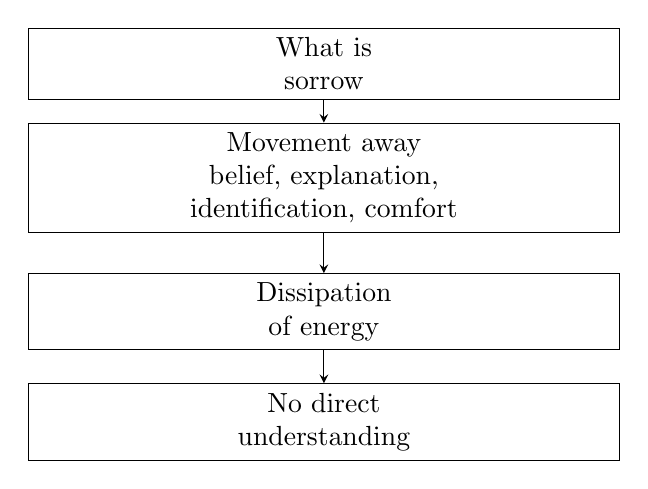
\begin{tikzpicture}[>=stealth]
\node[draw, align=center, text width=0.60\linewidth] (a) at (0,0) {What is\\sorrow};
\node[draw, align=center, text width=0.60\linewidth] (b) at (0,-1.45) {Movement away\\belief, explanation,\\identification, comfort};
\node[draw, align=center, text width=0.60\linewidth] (c) at (0,-3.15) {Dissipation\\of energy};
\node[draw, align=center, text width=0.60\linewidth] (d) at (0,-4.55) {No direct\\understanding};
\draw[->] (a) -- (b);
\draw[->] (b) -- (c);
\draw[->] (c) -- (d);
\end{tikzpicture}
\caption{Transcript-based reconstruction of escape from sorrow. The vertical shape keeps the causal order readable in a narrow format.}
\end{figure}

The point is not to rank escapes. A refined theological explanation and a crude distraction may be different in content, but both may function as movement away. The lecture's rigor lies here: the decisive question is not whether the explanation is noble, but whether the mind has moved from the fact.

\section{Non-Withdrawal and the Birth of Passion}

Once the structure of escape is clear, Krishnamurti states the converse. If the mind does not escape, does not rationalize, does not try to go beyond sorrow, and is not frightened of it, then it remains with sorrow. He gives ordinary examples: an incident, a word, an accident, a shattering sense of loneliness. The question is whether the mind can remain with such sorrow without movement away.

Let us introduce three labels only for clarity:

\begin{align}
E &= \text{escape from sorrow},\\
N &= \text{non-withdrawal from sorrow},\\
P &= \text{passion}.
\end{align}

Then the local logic of the passage is

\begin{align}
E &\Rightarrow \text{dissipated energy},\\
N &\Rightarrow P.
\end{align}

The second implication must remain cautious. It is not a technique. It does not say, perform \(N\) in order to acquire \(P\). Krishnamurti's point is that when the mind is no longer scattering itself in escape, passion is born. It is not artificial, not cultivated, and not the result of trying to be passionate.

\subsection{Question \& Answer}

\paragraph{Question.}
What happens when sorrow is not consoled, explained, or escaped?

\paragraph{Answer.}
Anderson brings in the word ``disconsolate.'' Ordinarily, we think the remedy is consolation, getting rid of the lack. Krishnamurti's answer reverses that reflex. If there is no escape and no desire to seek comfort away from what is, then out of that inescapable reality comes passion.

\begin{equation}
\text{no escape}
+
\text{remaining with sorrow}
\longrightarrow
\text{passion}.
\end{equation}

This is why beauty cannot be reduced to the appreciation of a painting or poem. One may write volumes on beauty or be a gifted artist, yet without this inward quality of passion, beauty remains indirect.

\begin{remark}
``Passion'' should not be allowed to drift into enthusiasm, excitement, emotional force, or appetite. In this lecture it is bound to sorrow, non-withdrawal, abandonment of the self, and austerity in the sense of inward simplicity.
\end{remark}

\section{Nature, Sensitivity, and Education}

The inquiry now turns outward again, but not back to objects as authorities. Krishnamurti speaks of lost contact with nature: the Grand Canyon admired and then left behind, a sunset treated as something merely happening, modern life driven outward by thought. The mind becomes artificial, superficial, verbal, and linear. Anderson's remark about the horizontal axis of success helps name the direction: always later, always more, always outward.

A compact contrast is

\begin{equation}
\text{linear pursuit}
\neq
\text{sensitive relation}.
\end{equation}

This is not a mathematical axis in the strict sense. It is a way of keeping the contrast visible. A life organized around success, money, position, and future gain may lose the delicacy through which beauty is perceived.

Krishnamurti then speaks of beauty in conduct: behaviour, language, voice, walking, humility, gentleness, quietness. This move is essential. Beauty is no longer confined to art, nature, or inward passion. It enters relationship and manner of living. If sensitivity of mind, heart, and body is lost, one cannot recover beauty by going somewhere to learn sensitivity as a technique.

The education passage follows directly. If beauty belongs to the whole movement of life, then education must be questioned. What are we being educated for? Merely to read, write, memorize, specialize, and become efficient? Or to understand fear, pleasure, relationship, order, beauty, care, and the whole field in which human beings live?

We can name that neglected field as

\begin{equation}
\mathcal{L}
=
\{\text{fear},\text{pleasure},\text{relationship},\text{order},
\text{beauty},\text{care}\}.
\end{equation}

The notation \(\mathcal{L}\) is only a bookkeeping device for the field of life. It helps us state the educational critique sharply:

\begin{equation}
\text{education as training}
\subsetneq
\text{education of the whole field } \mathcal{L}.
\end{equation}

The strict subset sign is schematic, not formal. It says that literacy, profession, technique, and information are not the whole of education. Krishnamurti's challenge is whether education can help a human being flower in beauty, goodness, affection, and care. Without that, the clever mind may still participate in the destruction of the earth and of relationship.

\section{What Is Action?}

After beauty, sorrow, passion, nature, sensitivity, and education, Krishnamurti makes the decisive turn: we must ask what action is. This is not a new topic but a tightening of the whole argument. Life is action. Speaking, sitting, discussing, and inquiring are all movements in action. Yet action as usually lived is mixed with regret, contradiction, repression, conformity, routine, repetition, and memory.

At this point the lecture gathers four terms into one field:

\begin{equation}
\mathcal{F}
=
\{\text{action},\text{sorrow},\text{passion},\text{beauty}\}.
\end{equation}

Krishnamurti explicitly warns against arranging them as a ladder: action at the beginning, beauty at the end. They are together. Still, to look carefully, he isolates action.

Ordinary action is action according to a formula, concept, ideology, belief, or pattern. The concept may be traditional, self-made, or supplied by an expert. It may be political, religious, or personal. The content varies, but the structure remains:

\begin{equation}
\text{ordinary action}
=
\text{action according to pattern}.
\end{equation}

More explicitly,

\begin{equation}
\text{perception}
\longrightarrow
\text{idea, belief, formula, conclusion}
\longrightarrow
\text{action}.
\end{equation}

This is mechanical action. Something is perceived; the mind draws from that perception an idea or conclusion; then action conforms to that mediator. Krishnamurti's criticism is that such action is removed from perception. It is action at a distance from seeing.

\begin{figure}
\centering
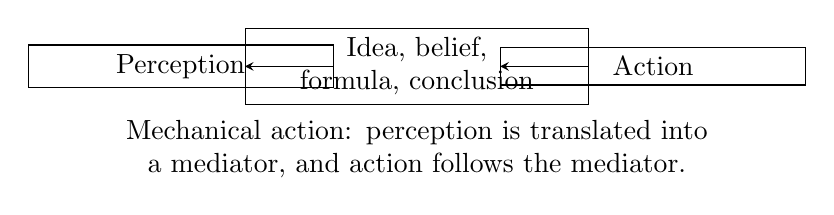
\begin{tikzpicture}[>=stealth]
\node[draw, align=center, text width=0.30\linewidth] (a) at (-3.0,0) {Perception};
\node[draw, align=center, text width=0.34\linewidth] (b) at (0,0) {Idea, belief,\\formula, conclusion};
\node[draw, align=center, text width=0.30\linewidth] (c) at (3.0,0) {Action};
\draw[->] (a) -- (b);
\draw[->] (b) -- (c);
\node[align=center, text width=0.78\linewidth] at (0,-1.05) {Mechanical action: perception is translated into a mediator, and action follows the mediator.};
\end{tikzpicture}
\caption{Transcript-based reconstruction of action according to idea.}
\end{figure}

\subsection{Question \& Answer}

\paragraph{Question.}
Can there be action without the idea?

\paragraph{Answer.}
This is the central question of the final movement. Krishnamurti notes that the word ``idea'' is connected with seeing, and then asks what we have done to seeing. Instead of seeing and doing, we see, draw a conclusion, and act according to the conclusion. The formula has inserted itself between perception and action.

The contrast is

\begin{align}
\text{mechanical action:}\quad
&\text{perception}
\rightarrow
\text{formula}
\rightarrow
\text{doing},\\
\text{free action:}\quad
&\text{seeing}
=
\text{doing}.
\end{align}

The equality sign is a compact rendering of Krishnamurti's phrase. It should not be read as a formal identity or a theory of psychology. It means that there is no interval in which the observer, as past, converts perception into a formula and then acts from the formula.

\subsection{A Worked Example: The Lag Between Idea and Action}

Krishnamurti says that between idea and action there is an interval, a lag of time, and that in that interval division and conflict enter. Let \(\Delta t\) denote that lag. The symbol is our notation; the distinction is his.

\begin{enumerate}
\item Perception is translated into an idea:
\begin{equation}
\text{perception}
\longrightarrow
\text{idea}.
\end{equation}

\item Action follows only after an interval:
\begin{equation}
\text{idea}
\xrightarrow{\Delta t}
\text{action}.
\end{equation}

\item During that interval, the action is no longer whole. Division has time to enter:
\begin{equation}
\Delta t > 0
\quad\Rightarrow\quad
\text{division enters}.
\end{equation}

\item Therefore action according to idea carries conflict:
\begin{equation}
\text{idea}
\xrightarrow{\Delta t}
\text{action}
\quad\Rightarrow\quad
\text{conflict}.
\end{equation}

\item The alternative is not a better idea but action without this mediation:
\begin{equation}
\Delta t = 0
\quad\text{in the limited sense that}\quad
\text{seeing is doing}.
\end{equation}
\end{enumerate}

The example is deliberately narrow. We are not measuring reaction time. We are tracking a distinction in the lecture: formula inserts psychological time; seeing as doing is action without that interval of translation.

\section{Seeing Is Doing}

The last movement names the mediator more exactly. The observer is not a neutral witness. In this passage the observer is the past, the formula, the concept, the belief. The observer comes between perception and doing. It is the factor of division.

We may write, as a shorthand,

\begin{equation}
\text{observer}
=
\text{past}
+
\text{formula}
+
\text{concept}
+
\text{belief}.
\end{equation}

This is not algebra. It is a compressed map of the terms Krishnamurti uses. The observer interrupts action:

\begin{equation}
\text{perception}
\longrightarrow
\text{observer}
\longrightarrow
\text{doing}.
\end{equation}

Against this, Krishnamurti places direct action:

\begin{equation}
\text{perception}
\longrightarrow
\text{doing}.
\end{equation}

\begin{figure}
\centering
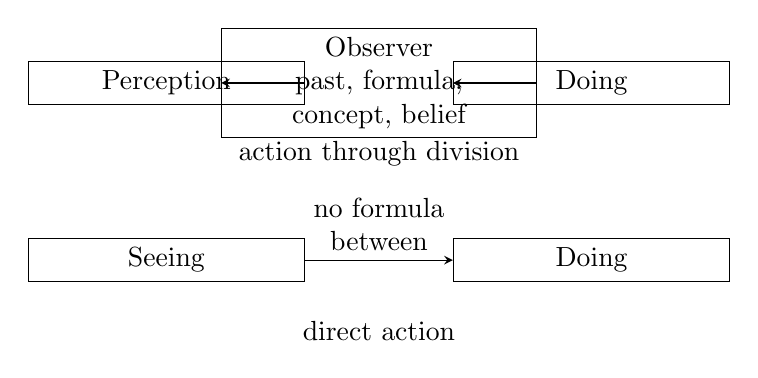
\begin{tikzpicture}[>=stealth]
\node[draw, align=center, text width=0.27\linewidth] (p1) at (-2.7,0) {Perception};
\node[draw, align=center, text width=0.31\linewidth] (o) at (0,0) {Observer\\past, formula,\\concept, belief};
\node[draw, align=center, text width=0.27\linewidth] (d1) at (2.7,0) {Doing};
\draw[->] (p1) -- (o);
\draw[->] (o) -- (d1);
\node[align=center] at (0,-0.9) {action through division};

\node[draw, align=center, text width=0.27\linewidth] (p2) at (-2.7,-2.25) {Seeing};
\node[draw, align=center, text width=0.27\linewidth] (d2) at (2.7,-2.25) {Doing};
\draw[->] (p2) -- node[above, align=center] {no formula\\between} (d2);
\node[align=center] at (0,-3.15) {direct action};
\end{tikzpicture}
\caption{Transcript-based reconstruction of the distinction between action through the observer and action as seeing-doing.}
\end{figure}

Krishnamurti's concrete example is danger at the edge of a precipice. Seeing danger is instant action. One does not first construct an idea of danger, compare it with an ideology of cliffs, and then act. The seeing is already the movement. At the same time, he immediately notes that we are conditioned both to physical danger and to the belief that action requires formula. The example is therefore not simplistic. It shows that direct action is intelligible, while also showing how deeply the mind is conditioned to mediation.

The final autobiographical example has the same structure. A large spiritual organization had formed around Krishnamurti. In 1928 he saw that it was wrong, dissolved it, and returned the property. The point is not biographical display. It is an instance of action without comparison, conclusion, dependence, or regret: he saw and acted.

\section{Summary}

The lecture begins by questioning beauty as something stored in museums, paintings, poems, cathedrals, and expert accounts. It then turns inward: beauty cannot be understood without passion, and passion is born when the mind does not withdraw from sorrow. This does not mean that suffering is to be cultivated. It means that escape from sorrow dissipates the energy needed to understand what is.

The inquiry then widens into nature, sensitivity, conduct, education, and civilization. A life organized around success, money, position, and verbal knowledge may lose sensitivity in the mind, heart, body, speech, and relationship. Education becomes suspect when it trains skill and knowledge while omitting fear, pleasure, relationship, order, beauty, and care.

The final turn is action. Ordinary action follows idea, formula, pattern, memory, or ideology. Such action is mechanical because it is removed from perception. Krishnamurti's alternative is compressed in the phrase

\begin{equation}
\text{seeing} = \text{doing}.
\end{equation}

The chapter's conceptual spine is therefore a sequence of distinctions: expression is not beauty; escape is not understanding; cultivated passion is not passion; training is not the education of the whole field of life; action according to idea is not free action. What remains is the possibility that, when the observer as past does not intervene, perception itself is action.